%%%%%%%%%%%%%%%%%%%%%%%%%%%%%%%%%%%%%%%%%%%%%%%%%%%%%%%%%%%%%%%%%%%%%%%%%%%%%%%%%%%%%%%%%%%%%%%%
%
% CSCI 1430 Written Question Template
%
% This is a LaTeX document. LaTeX is a markup language for producing documents.
% Your task is to answer the questions by filling out this document, then to
% compile this into a PDF document.
%
% TO COMPILE:
% > pdflatex thisfile.tex

% If you do not have LaTeX, your options are:
% - VSCode extension: https://marketplace.visualstudio.com/items?itemName=James-Yu.latex-workshop
% - Online Tool: https://www.overleaf.com/ - most LaTeX packages are pre-installed here (e.g., \usepackage{}).
% - Personal laptops (all common OS): http://www.latex-project.org/get/ 
%
% If you need help with LaTeX, please come to office hours.
% Or, there is plenty of help online:
% https://en.wikibooks.org/wiki/LaTeX
%
% Good luck!
% The CSCI 1430 staff
%
%%%%%%%%%%%%%%%%%%%%%%%%%%%%%%%%%%%%%%%%%%%%%%%%%%%%%%%%%%%%%%%%%%%%%%%%%%%%%%%%%%%%%%%%%%%%%%%%
%
% How to include two graphics on the same line:
% 
% \includegraphics[width=0.49\linewidth]{yourgraphic1.png}
% \includegraphics[width=0.49\linewidth]{yourgraphic2.png}
%
% How to include equations:
%
% \begin{equation}
% y = mx+c
% \end{equation}
% 
%%%%%%%%%%%%%%%%%%%%%%%%%%%%%%%%%%%%%%%%%%%%%%%%%%%%%%%%%%%%%%%%%%%%%%%%%%%%%%%%%%%%%%%%%%%%%%%%

\documentclass[10pt,twocolumn,letterpaper]{article}
 
\usepackage{cvpr}
\usepackage{times}
\usepackage{epsfig}
\usepackage{graphicx}
\usepackage{amsmath}
\usepackage{amssymb}
\usepackage{booktabs}
\usepackage{microtype}
% From https://ctan.org/pkg/matlab-prettifier
\usepackage[numbered,framed]{matlab-prettifier}

\frenchspacing

% Include other packages here, before hyperref.

% If you comment hyperref and then uncomment it, you should delete
% egpaper.aux before re-running latex.  (Or just hit 'q' on the first latex
% run, let it finish, and you should be clear).
\usepackage[pagebackref=true,breaklinks=true,letterpaper=true,colorlinks,bookmarks=false]{hyperref}

\cvprfinalcopy
\def\cvprPaperID{****}
\def\httilde{\mbox{\tt\raisebox{-.5ex}{\symbol{126}}}}
\ifcvprfinal\pagestyle{empty}\fi

\begin{document}

%%%%%%%%% TITLE
\title{CSCI 1430 Final Project Report:\\Sailboat Pose Estimation from Drone Footage}

% Make this document not anonymous
\author{
    \emph{Team name}: Quinn Brighton, Nishani Clarke, Alexandra McIntyre.\\
    \emph{TA name:} Kelvin Jiang.
    Brown University\\
}

\maketitle
%\thispagestyle{empty}

%%%%%%%%% ABSTRACT
\begin{abstract}
Recovering the 3D geometry of sailboat races from monocular drone footage is challenging due to changing viewpoints, occlusion, water reflections, and the absence of camera calibration or GPS measurements. We present a pipeline for metric sailboat pose estimation using a frozen DINOv3 visual backbone, lightweight learned keypoint heads, and a geometric optimization solver. Our method predicts four keypoints per boat --- mast top, mast base, bow, and stern --- through a staged conditioning pipeline consisting of a CNN tip detector followed by transformer-based base and hull predictors. These image-space detections are then used in a single-frame reprojection solver that jointly estimates camera pose and per-boat 3D position, orientation, and heel angle using known sailboat geometry. To improve robustness, the solver iteratively removes high-error outlier keypoints before final refinement. On out-of-sample regatta footage, our system recovers six boats simultaneously with approximately 2.5-pixel reprojection accuracy on 1080p imagery while producing metrically-scaled top-down reconstructions of the race.
\end{abstract}


\section{Project Report Advice [Delete This Section]}

\begin{enumerate}
    \item Overriding principle: show us your effort.
    \item If you wish us to consider any aspect of your project, it should be presented here. \item Please include a problem statement, related work, your method, your results (figures! tables!), any comparison to existing techniques, and references. 
    \item If you made something work---great! If you didn't quite make it work---tell us about the problems, why you think it didn't work, and what you would do to fix it.
    \item Length: Approximately four pages for techical description. For social impact, no more than one page total.
    \item Please include an appendix to the report which details what each team member contributed to the project. One paragraph max each.
    \item Any other materials should go in an appendix.
\end{enumerate}


%%%%%%%%% BODY TEXT
\section{Introduction}

\section{Introduction}

In recent years, many major sports have adopted advanced analytics and player tracking systems to better understand strategy, optimize performance, and visualize gameplay. Professional leagues such as the NFL, NBA, and NHL now rely heavily on spatial tracking data to analyze positioning, movement, and tactical decision making. Collegiate sailing, however, still lacks comparable tools despite the strategic complexity of team racing. At most regattas, coaches and sailors collect hundreds of hours of drone footage, but reviewing this footage manually is time-consuming and makes it difficult to consistently analyze boat positioning and race dynamics over time.

As collegiate sailors ourselves, we were motivated by the idea of making team racing strategy more visible and understandable. Our goal is to determine whether monocular drone footage can be converted into a standardized top-down representation of a race, enabling quantitative analysis of positioning, tactics, and fleet movement. Such a system could eventually support coaching tools, automated race visualization, and large-scale statistical analysis of sailing strategy.

Recovering sailboat pose from drone footage presents several significant challenges. Boats appear at widely varying scales and orientations depending on camera angle, distance, and heel. Water reflections, wakes, sail occlusions, and overlapping boats further complicate visual detection. In addition, the drone camera itself is constantly moving, and no calibrated camera parameters or ground-truth GPS measurements are available. This makes estimating both boat pose and camera pose from a single frame an inherently underconstrained problem.

To address these challenges, we develop a pipeline that combines self-supervised visual features, lightweight learned keypoint predictors, and geometric optimization. We first use a frozen DINOv3 visual transformer backbone to extract dense image features from each frame. On top of these features, we train a sequence of lightweight neural heads that predict four keypoints per boat: mast top, mast base, bow, and stern. These detections are then passed into a geometric solver that jointly estimates camera parameters and metric boat pose by minimizing reprojection error under a known sailboat geometry model. To improve robustness, the solver iteratively removes high-error outlier detections before final refinement.

Our results demonstrate that monocular drone footage can be used to recover metrically-scaled sailboat pose with low reprojection error, suggesting that automated spatial analysis of team racing is feasible using existing regatta recordings.

\section{Related Work}

Cite and discuss work that you used in your project, including any software used. Citations are written into a .bib file in BibTeX format, and can be called like this: Alpher et al.~\cite{Alpher04}. Here's a brief intro: \href{http://www.andy-roberts.net/writing/latex/bibliographies}{webpage}. \emph{Hint:} \$$>$ pdflatex \%docu, bibtex \%docu, pdflatex \%docu, pdflatex \%docu

Lorem ipsum dolor sit amet, consectetur adipiscing elit, sed do eiusmod tempor incididunt ut labore et dolore magna aliqua. Ut enim ad minim veniam, quis nostrud exercitation ullamco laboris nisi ut aliquip ex ea commodo consequat. Duis aute irure dolor in reprehenderit in voluptate velit esse cillum dolore eu fugiat nulla pariatur. Excepteur sint occaecat cupidatat non proident, sunt in culpa qui officia deserunt mollit anim id est laborum. Watch for hanging orphans; they make a document look ugly.

\section{Method}

Our goal is to recover a metrically-scaled top-down representation of a sailing race from monocular drone footage. Given a single drone frame, our pipeline predicts four semantic keypoints for each sailboat --- mast top, mast base, bow, and stern --- and uses these detections to estimate both camera pose and boat pose in a shared 3D world coordinate system.

Our method consists of two major stages: a learned keypoint detection pipeline built on frozen DINOv3 features, and a geometric optimization solver that reconstructs the scene from the detected image-space keypoints. Figure~\ref{fig:pipeline} shows an overview of the full pipeline.

\subsection{DINOv3 Feature Extraction}

We use a frozen DINOv3 Vision Transformer backbone as the visual feature extractor for all downstream tasks. Specifically, we use the \texttt{facebook/dinov3-vits16-pretrain-lvd1689m} model, which produces dense 384-dimensional feature embeddings for overlapping image patches. The backbone is never fine-tuned during training.

Each input frame is resized so that the longest image dimension is at most 1808 pixels and both spatial dimensions are divisible by 16. Images are normalized using ImageNet statistics before being passed through the network. We modify the patch embedding stride from the default 16 pixels to 8 pixels, producing overlapping patches and a denser spatial feature grid. This significantly improves localization accuracy for small structures such as sailboat masts.

After inference, the transformer tokens are reshaped into a dense spatial feature tensor:
\begin{equation}
F \in \mathbb{R}^{H \times W \times 384},
\end{equation}
where each spatial cell contains a normalized 384-dimensional feature vector. These dense features are cached and reused by all later stages of the pipeline.

\subsection{Stage 1: Mast Tip Detection}

The first stage of the pipeline identifies mast top locations within the image. We train a lightweight convolutional neural network called \texttt{TileHead} that operates on local windows of DINOv3 features and predicts a heatmap indicating the probability of a mast tip at each spatial cell.

The network consists of several convolutional layers with ReLU activations and produces a single-channel output heatmap. During training, Gaussian heatmaps centered on labeled mast tips are used as targets. The model is trained using binary cross entropy loss on both positive and hard negative image tiles.

At inference time, the network is applied densely across the feature grid using a sliding-window approach. Predicted heatmaps are merged into a global confidence map and clustered using DBSCAN to produce a final set of mast tip detections. These detections are then mapped back into source-image pixel coordinates.

\subsection{Stage 2: Tip-Conditioned Mast Base Prediction}

Given a detected mast tip, the second stage predicts the corresponding mast base location. Unlike the tip detector, this task requires reasoning over larger spatial distances and understanding the global structure of the sailboat. To accomplish this, we use a transformer-based architecture called \texttt{TipAttnBaseHead}.

For each detected mast tip, we extract a local feature window centered around the tip location. The mast tip is pinned to a fixed position within the window, allowing the network to learn consistent spatial relationships between the mast top and mast base. The extracted features are projected into a lower-dimensional embedding space, augmented with two-dimensional positional encodings, and processed using a multi-layer transformer encoder.

After transformer processing, the feature vector corresponding to the mast tip is concatenated with every spatial feature in the window. A small multilayer perceptron then predicts a spatial heatmap representing the probability of the mast base location.

The output heatmap is converted into a sub-pixel base prediction using a weighted centroid around the maximum response.

\subsection{Stage 3: Bow and Stern Prediction}

The final learned stage predicts the bow and stern locations for each detected sailboat. This stage uses both the mast tip and mast base as conditioning signals, since the relationship between the mast and hull orientation provides important information about boat heading and heel direction.

We use a second transformer-based architecture, \texttt{TipBaseBowSternAttnHead}, which shares the same general structure as the mast-base predictor. A local feature window is extracted around the detected mast tip, and the transformer processes the full spatial context of the boat.

Instead of conditioning only on the mast tip feature, this network combines the transformer embeddings at both the mast tip and mast base locations. The resulting conditioning vector is concatenated with every spatial token before prediction. The network outputs two heatmaps simultaneously: one for the bow and one for the stern.

For each detected sailboat, the output of the learned pipeline is a set of four image-space keypoints:
\begin{equation}
K_i = \{ \mathbf{u}_{\text{bow}}, \mathbf{u}_{\text{stern}}, \mathbf{u}_{\text{base}}, \mathbf{u}_{\text{tip}} \}.
\end{equation}

\subsection{Single-Frame Geometric Solver}

The predicted image-space keypoints are passed into a geometric optimization solver that reconstructs the 3D scene from a single image. Our solver jointly estimates camera parameters and per-boat pose parameters by minimizing reprojection error.

We model each sailboat using a rigid metric template with known physical dimensions corresponding to collegiate FJ and 420 sailboats. The boat model includes four semantic landmarks: bow, stern, mast base, and mast top. Because mast height and hull length are known, the optimization problem becomes metrically constrained.

The world coordinate system is defined such that the water surface lies on the plane:
\begin{equation}
z = 0.
\end{equation}

The unknown optimization variables include camera pitch, yaw, height, focal length, and horizontal position, along with each boat's planar position, yaw, and heel angle.

For each boat landmark, the solver projects the corresponding 3D point into image space using a pinhole camera model:
\begin{equation}
\hat{\mathbf{u}}_{i,j} = \Pi(\mathbf{X}_{i,j}; \theta_{\text{cam}}, \theta_i^{\text{boat}}),
\end{equation}
where $\Pi$ denotes the projection function, $\theta_{\text{cam}}$ represents the camera parameters, and $\theta_i^{\text{boat}}$ represents the pose parameters of boat $i$.

Optimization minimizes reprojection error between predicted and observed image-space keypoints:
\begin{equation}
E_{\text{reproj}} =
\sum_{i,j}
\left\|
\hat{\mathbf{u}}_{i,j}
-
\mathbf{u}_{i,j}
\right\|_2^2.
\end{equation}

To stabilize optimization under ambiguous viewpoints, we include a soft prior on sailboat heel angles. Large heel values are weakly penalized unless strongly supported by image evidence.

\subsection{Iterative Outlier Rejection}

Predicted keypoints occasionally contain large localization errors due to occlusion, overlapping sails, or poor visibility. To improve robustness, we introduce an iterative outlier rejection procedure.

After each optimization pass, reprojection errors are evaluated independently for every keypoint. The highest-error keypoint exceeding a predefined threshold is removed from the active optimization set, and the solver is rerun. This process continues until all remaining keypoints fall below the error threshold or each boat reaches a minimum number of active landmarks.

Finally, a last optimization pass is performed with the heel prior enabled to regularize any remaining ambiguity in the reconstruction.

\section{Results}

We evaluated our pipeline on out-of-sample drone footage containing both collegiate 420 and FJ sailboats under varying viewing angles and environmental conditions. Our primary goal was to determine whether monocular drone footage could be transformed into a stable, metrically-scaled representation of team race dynamics.

\subsection{Keypoint Detection Performance}

After training on approximately 200 manually labeled samples, the first-stage mast tip detector achieved near-perfect detection accuracy on out-of-sample frames drawn from the same regatta footage. The frozen DINOv3 backbone produced highly separable spatial features for sails, boats, and water regions, allowing the lightweight CNN tip detector to localize mast tops reliably despite changing camera perspectives and partial occlusions.

Using the mast tip detections as conditioning signals, the subsequent transformer-based stages successfully predicted mast base, bow, and stern positions for each detected sailboat. Figure~\ref{fig:result1} shows an example out-of-sample frame with the predicted semantic keypoints overlaid on multiple boats simultaneously.

The sequential conditioning structure of the pipeline proved important for stable localization. Predicting mast base locations relative to the detected mast tip significantly reduced ambiguity compared to attempting to predict all keypoints independently. Similarly, conditioning bow and stern prediction on both mast top and mast base information improved orientation consistency across varying heel angles and viewing directions.

\begin{figure}[t]
    \centering
    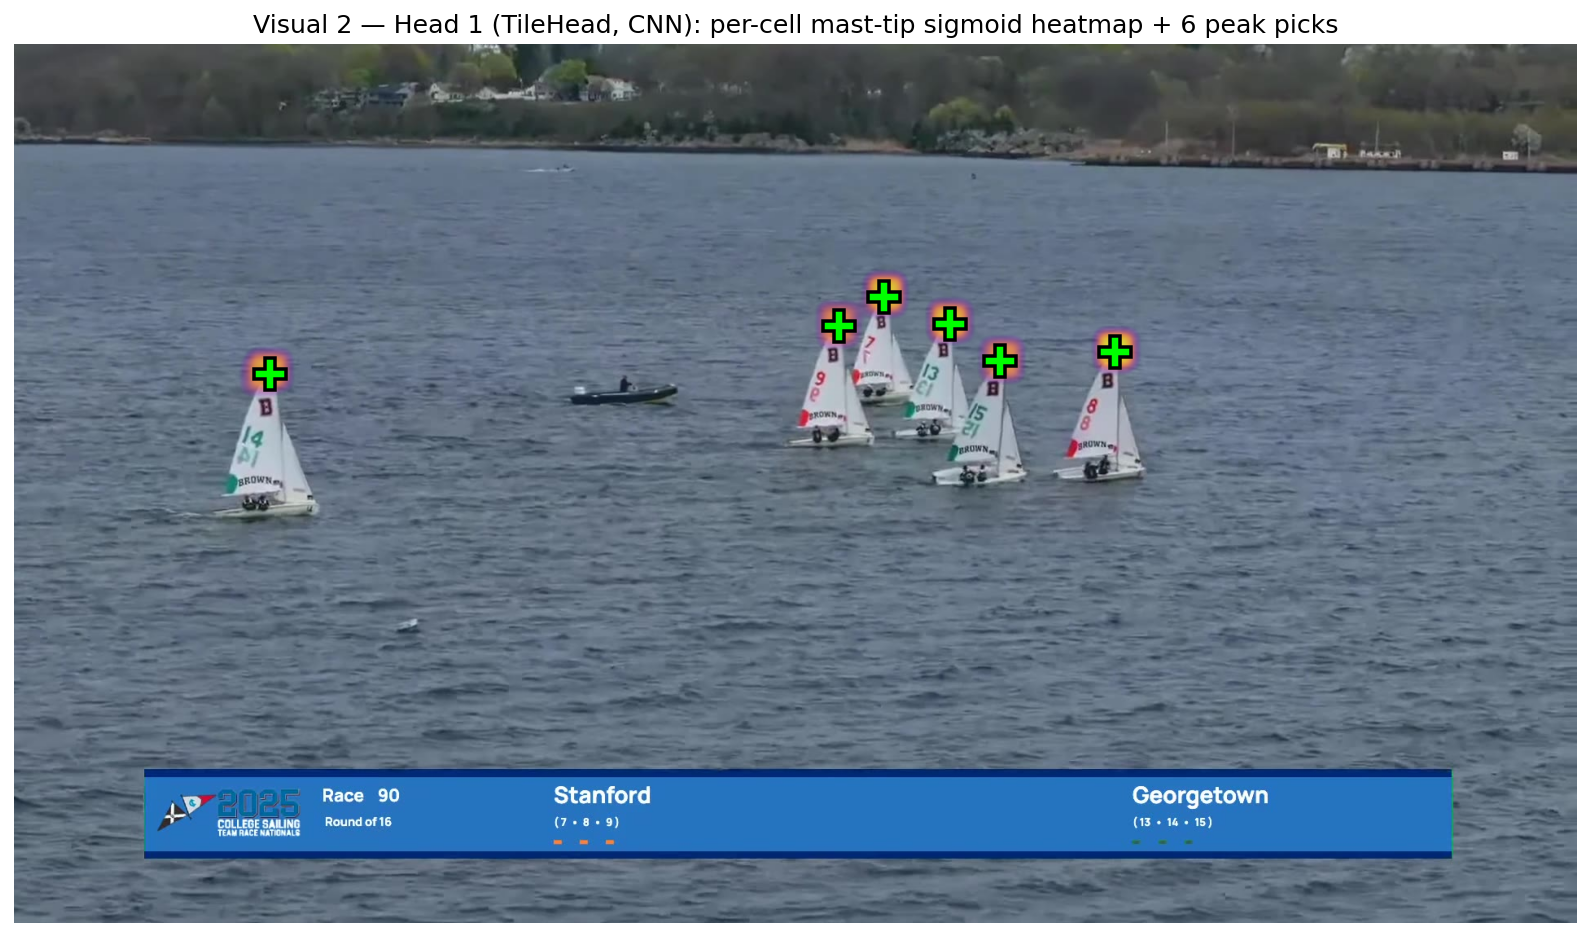
\includegraphics[width=\linewidth]{02_tip_heatmap.png}
    \caption{Single-wide figure.}
    \label{fig:result1}
\end{figure}

\subsection{Single-Frame Geometric Reconstruction}

The predicted keypoints were passed into the single-frame optimization solver to estimate camera pose and metrically-scaled boat positions. Using known hull and mast dimensions for collegiate sailboats, the solver jointly optimized camera parameters and per-boat pose variables by minimizing reprojection error between the observed and predicted image-space keypoints.

On representative out-of-sample frames containing six boats, the solver achieved low reprojection error while producing visually consistent top-down reconstructions of the fleet. The iterative outlier rejection procedure substantially improved robustness in frames containing partially occluded sails or noisy detections. High-error keypoints were removed prior to final optimization, preventing individual failures from distorting the recovered scene geometry.

Figure~\ref{fig:result2} shows an example reconstruction result. The left image shows the original drone frame with predicted keypoints, while the right image visualizes the reconstructed top-down metric boat positions.

\subsection{Temporal Boat Trajectory Estimation}

To estimate boat motion over time, we chained together the optimized single-frame reconstructions across sequential video frames. The single-frame solver produced an initial estimate of boat pose in each frame, and these estimates were merged into continuous trajectories across time.

Before temporal merging, outlier detections identified during the single-frame optimization stage were removed to preserve trajectory consistency and reduce instability. This was particularly important in cases where boats overlapped visually or when portions of a mast or hull became temporarily occluded.

The resulting trajectories produced a stable two-dimensional representation of fleet movement throughout the race sequence. These reconstructions demonstrate the feasibility of recovering approximate team-racing dynamics and spatial positioning directly from monocular drone footage without GPS measurements or calibrated camera systems.

\begin{table}[t]
\begin{center}
\begin{tabular}{l c}
\toprule
Metric & Result \\
\midrule
Training samples & 200 \\
Boat classes & FJ, 420 \\
Mast tip detection accuracy & Near 100\% \\
Solver type & Monocular geometric optimization \\
Outlier handling & Iterative rejection \\
Output representation & Metric 2D trajectories \\
\bottomrule
\end{tabular}
\end{center}
\caption{Summary of qualitative and quantitative results from the sailboat pose estimation pipeline.}
\label{tab:results}
\end{table}
Lorem ipsum dolor sit amet, consectetur adipiscing elit, sed do eiusmod tempor incididunt ut labore et dolore magna aliqua. Ut enim ad minim veniam, quis nostrud exercitation ullamco laboris nisi ut aliquip ex ea commodo consequat. Duis aute irure dolor in reprehenderit in voluptate velit esse cillum dolore eu fugiat nulla pariatur. Excepteur sint occaecat cupidatat non proident, sunt in culpa qui officia deserunt mollit anim id est laborum.

\begin{figure*}[t]
    \centering
    
\includegraphics[width=0.4\linewidth]{placeholder.jpg}
    
\includegraphics[width=0.4\linewidth]{placeholder.jpg}
    \caption{Double-wide figure. \emph{Left:} My result was spectacular. \emph{Right:} Curious.}
    \label{fig:result2}
\end{figure*}

Lorem ipsum dolor sit amet, consectetur adipiscing elit, sed do eiusmod tempor incididunt ut labore et dolore magna aliqua. Ut enim ad minim veniam, quis nostrud exercitation ullamco laboris nisi ut aliquip ex ea commodo consequat. Duis aute irure dolor in reprehenderit in voluptate velit esse cillum dolore eu fugiat nulla pariatur. Excepteur sint occaecat cupidatat non proident, sunt in culpa qui officia deserunt mollit anim id est laborum.

%-------------------------------------------------------------------------
\subsection{Technical Discussion}

What about your method raises interesting questions? Are there any trade-offs? What is the right way to think about the changes that you made?

Lorem ipsum dolor sit amet, consectetur adipiscing elit, sed do eiusmod tempor incididunt ut labore et dolore magna aliqua. Ut enim ad minim veniam, quis nostrud exercitation ullamco laboris nisi ut aliquip ex ea commodo consequat. Duis aute irure dolor in reprehenderit in voluptate velit esse cillum dolore eu fugiat nulla pariatur. Excepteur sint occaecat cupidatat non proident, sunt in culpa qui officia deserunt mollit anim id est laborum.

%------------------------------------------------------------------------
\section{Conclusion}

What you did, why it matters, what the impact is going forward.

{\small
\bibliographystyle{plain}
\bibliography{ProjectFinal_ProjectReportTemplate}
}

\section*{Appendix}

\subsection*{Team contributions}

Please describe in one paragraph per team member what each of you contributed to the project.
\begin{description}
\item[Person 1 (put your real names)] Lorem ipsum dolor sit amet, consectetur adipiscing elit, sed do eiusmod tempor incididunt ut labore et dolore magna aliqua. Ut enim ad minim veniam, quis nostrud exercitation ullamco laboris nisi ut aliquip ex ea commodo consequat. Duis aute irure dolor in reprehenderit in voluptate velit esse cillum dolore eu fugiat nulla pariatur. 
\item[Person 2 (put your real names)] Lorem ipsum dolor sit amet, consectetur adipiscing elit, sed do eiusmod tempor incididunt ut labore et dolore magna aliqua. Ut enim ad minim veniam, quis nostrud exercitation ullamco laboris nisi ut aliquip ex ea commodo consequat. Duis aute irure dolor in reprehenderit in voluptate velit esse cillum dolore eu fugiat nulla pariatur.
\item [Person 3 (put your real names)] Lorem ipsum dolor sit amet, consectetur adipiscing elit, sed do eiusmod tempor incididunt ut labore et dolore magna aliqua. Ut enim ad minim veniam, quis nostrud exercitation ullamco laboris nisi ut aliquip ex ea commodo consequat. Duis aute irure dolor in reprehenderit in voluptate velit esse cillum dolore eu fugiat nulla pariatur. 
\item [Person 4 (put your real names)] Lorem ipsum dolor sit amet, consectetur adipiscing elit, sed do eiusmod tempor incididunt ut labore et dolore magna aliqua. Ut enim ad minim veniam, quis nostrud exercitation ullamco laboris nisi ut aliquip ex ea commodo consequat. Duis aute irure dolor in reprehenderit in voluptate velit esse cillum dolore eu fugiat nulla pariatur.
\end{description}

\end{document}
